\subsection{Differences in Choice of $g(x)$}
Below are three plots used to determine the best choice for $g(x)$ when factorizing a number consisting of two prime factors. A lower value refers to lower time taken, which is considered better. The figure \ref{fig:pollardsAllModes} displays all tested functions - $g(x)=x^2+1$ in blue, $g(x)=x^3+1$ in red, $g(x)=x^2+3$ in green and $g(x)=x+1$ in orange. Figure \ref{fig:pollardsFasterModes} shows only the three fastest modes tested - not including $g(x)=x+1$. The figure \ref{fig:pollardsFastestModes} shows only the two fastest choices of $g(x)$ - $g(x)=x^2+1$ and $g(x)=x^3+1$.

\begin{figure}[H]
    \centering
    \begin{tikzpicture}[scale=0.6, trim axis left, trim axis right]
\begin{axis}[
    width=1\textwidth,
    height=1\textwidth,
    xmin=1.0, xmax=24,
    ymin=1.4e-05, ymax=203.875711333,
    xlabel={Number of bits},
    ylabel={Time taken (s)},
    xticklabels={2, , 4, , 6, , 8, , 10, , 12, , 14, , 16, , 18, , 20, , 22, },
    xtick={2, 3, 4, 5, 6, 7, 8, 9, 10, 11, 12, 13, 14, 15, 16, 17, 18, 19, 20, 21, 22, 23},
    ytick={0.0000140000000000000, 20.3875837333000, 40.7751534666000, 61.1627231999000, 81.5502929332000, 101.937862666500, 122.325432399800, 142.713002133100, 163.100571866400, 183.488141599700},
    x tick label style={rotate=45, anchor=east, align=right,text},
    ymajorgrids=true,
    grid style=dashed,
]

%%%%
%% default
%%%%

\addplot+[
    blue,
    very thick,
    forget plot,
    only marks
    ]
    plot[
    very thick,
    error bars/.cd,
    y dir=plus,
    y explicit
    ]
    table[x=x,y=y,y error expr=\thisrow{y-max}] {
    x    y    y-max
20	0.01139255	0.01163245
21	0.0064126	0.0007144
22	0.0120458	0.0002592
23	0.00549895	0.00021005
3	4.275e-05	0.00025425
5	0.0001019	0.0002861
4	7.175e-05	0.00031025
7	0.0001121	0.0002729
6	0.0001007	0.0002753
9	0.00019415	0.00019985
8	0.000156	0.000302
11	0.0001366	0.0001954
10	0.00041435	0.00021065
13	0.0010869	0.0002211
12	0.0001853	0.0002137
15	0.00211385	0.00021415
14	0.00121215	0.00020285
17	0.006028	0.000198
16	0.0014122	0.0006718
19	0.00454975	0.00041425
18	0.0023315	0.0002405

    };

\addplot+[
    blue,
    very thick,
    forget plot,
    only marks
    ]
    plot[
    very thick,
    error bars/.cd,
    y dir=plus,
    y explicit
    ]
    table[x=x,y=y,y error expr=\thisrow{y-min}] {
    x    y    y-min
20	0.01139255	-0.00103755
21	0.0064126	-7.76e-05
22	0.0120458	-6.88e-05
23	0.00549895	-6.695e-05
3	4.275e-05	-1.975e-05
5	0.0001019	-3.49e-05
4	7.175e-05	-3.375e-05
7	0.0001121	-2.71e-05
6	0.0001007	-3.27e-05
9	0.00019415	-2.515e-05
8	0.000156	-1.7e-05
11	0.0001366	-2.36e-05
10	0.00041435	-2.935e-05
13	0.0010869	-3.79e-05
12	0.0001853	-2.53e-05
15	0.00211385	-4.385e-05
14	0.00121215	-3.315e-05
17	0.006028	-5e-05
16	0.0014122	-8.22e-05
19	0.00454975	-7.575e-05
18	0.0023315	-4.45e-05

    };

%%%%
%% higher
%%%%

\addplot+[
    red,
    very thick,
    forget plot,
    only marks
    ]
    plot[
    very thick,
    error bars/.cd,
    y dir=plus,
    y explicit
    ]
    table[x=x,y=y,y error expr=\thisrow{y-max}] {
    x    y    y-max
    24	0.049109	0.000762
20	1.6806099	0.0517161
21	0.01877765	0.00039335
22	0.04212975	0.00885625
23	64.5804449	0.2069811
3	5.775e-05	0.00051125
2	4.05e-05	0.0002325
5	6.26e-05	0.0002234
4	7.055e-05	0.00021245
7	0.00015215	0.00020485
6	7.735e-05	0.00020765
9	0.00459855	0.00064245
8	6.52e-05	0.0002048
11	0.0003642	0.0004108
10	0.00012745	0.00028655
13	0.0132486	0.0010574
12	0.0002597	0.0004113
15	0.06393975	0.01271525
14	0.000113	0.000231
17	0.00078135	0.00022465
16	1.19460925	0.04708275
19	0.00730095	0.00025605
18	0.51693845	0.00763255

    };

\addplot+[
    red,
    very thick,
    forget plot,
    only marks
    ]
    plot[
    very thick,
    error bars/.cd,
    y dir=plus,
    y explicit
    ]
    table[x=x,y=y,y error expr=\thisrow{y-min}] {
    x    y    y-min
    24	0.049109	-0.000328
20	1.6806099	-0.0165949
21	0.01877765	-0.00025365
22	0.04212975	-0.00194175
23	64.5804449	-0.1968029
3	5.775e-05	-3.675e-05
2	4.05e-05	-2.65e-05
5	6.26e-05	-2.36e-05
4	7.055e-05	-2.455e-05
7	0.00015215	-1.515e-05
6	7.735e-05	-2.335e-05
9	0.00459855	-0.00018655
8	6.52e-05	-1.22e-05
11	0.0003642	-0.0001192
10	0.00012745	-4.945e-05
13	0.0132486	-0.0002546
12	0.0002597	-7.47e-05
15	0.06393975	-0.00180575
14	0.000113	-1.3e-05
17	0.00078135	-3.235e-05
16	1.19460925	-0.01094925
19	0.00730095	-0.00010295
18	0.51693845	-0.00232645

    };

%%%%
%% odd
%%%%

\addplot+[
    green,
    very thick,
    forget plot,
    only marks
    ]
    plot[
    very thick,
    error bars/.cd,
    y dir=plus,
    y explicit
    ]
    table[x=x,y=y,y error expr=\thisrow{y-max}] {
    x    y    y-max
    24	0.0693093	0.0004957
20	0.0038716	0.0002414
21	0.0127793	0.0001607
22	0.0262544	0.0001926
23	0.045302	0.001481
3	5.51e-05	0.0002409
5	7.17e-05	0.0002293
4	6.41e-05	0.0001939
7	8.91e-05	0.0002279
6	0.0001654	0.0002266
9	0.00017	0.000228
8	9.05e-05	0.0002355
11	0.0003966	0.0001944
10	0.0001904	0.0001926
13	0.0008766	0.0001904
12	0.0005937	0.0002313
15	0.0022656	0.0003534
14	0.0007608	0.0001902
17	0.0004967	0.0002183
16	0.0049573	0.0002257
19	0.0084545	0.0002855
18	0.0079593	0.0020017

    };

\addplot+[
    green,
    very thick,
    forget plot,
    only marks
    ]
    plot[
    very thick,
    error bars/.cd,
    y dir=plus,
    y explicit
    ]
    table[x=x,y=y,y error expr=\thisrow{y-min}] {
    x    y    y-min
    24	0.0693093	-0.0003953
20	0.0038716	-3.96e-05
21	0.0127793	-4.13e-05
22	0.0262544	-0.0001674
23	0.045302	-0.000448
3	5.51e-05	-2.71e-05
5	7.17e-05	-2.57e-05
4	6.41e-05	-2.51e-05
7	8.91e-05	-2.61e-05
6	0.0001654	-2.74e-05
9	0.00017	-2.7e-05
8	9.05e-05	-2.65e-05
11	0.0003966	-2.36e-05
10	0.0001904	-2.24e-05
13	0.0008766	-2.96e-05
12	0.0005937	-2.97e-05
15	0.0022656	-5.96e-05
14	0.0007608	-2.58e-05
17	0.0004967	-2.87e-05
16	0.0049573	-7.23e-05
19	0.0084545	-6.45e-05
18	0.0079593	-0.0004983

    };

%%%%
%% trial
%%%%

\addplot+[
    orange,
    very thick,
    forget plot,
    only marks
    ]
    plot[
    very thick,
    error bars/.cd,
    y dir=plus,
    y explicit
    ]
    table[x=x,y=y,y error expr=\thisrow{y-max}] {
    x    y    y-max
    24	203.875711333	0.217778666667
20	11.5883435	0.0471235
21	22.3785966	0.0549324
22	39.0804425	0.1148155
23	129.0535278	0.1520112
3	9.7e-05	0.000219
2	7.52e-05	0.0002358
5	0.0003765	0.0002225
4	0.0001594	0.0002436
7	0.0014637	0.0001813
6	0.0007246	0.0002034
9	0.0052146	0.0015024
8	0.0021437	0.0010213
11	0.0149539	0.0013661
10	0.0084726	0.0002154
13	0.0638937	0.0003233
12	0.0425776	0.0053524
15	0.4380419	0.0023671
14	0.143031	0.004182
17	1.3133083	0.0352727
16	1.1396995	0.0338595
19	8.1233323	0.1003857
18	2.6604783	0.0377227

    };

\addplot+[
    orange,
    very thick,
    forget plot,
    only marks
    ]
    plot[
    very thick,
    error bars/.cd,
    y dir=plus,
    y explicit
    ]
    table[x=x,y=y,y error expr=\thisrow{y-min}] {
    x    y    y-min
    24	203.875711333	-0.161111333333
20	11.5883435	-0.0500685
21	22.3785966	-0.0431876
22	39.0804425	-0.0945705
23	129.0535278	-0.3061288
3	9.7e-05	-2.5e-05
2	7.52e-05	-2.72e-05
5	0.0003765	-2.95e-05
4	0.0001594	-2.94e-05
7	0.0014637	-3.97e-05
6	0.0007246	-3.56e-05
9	0.0052146	-0.0003446
8	0.0021437	-0.0001797
11	0.0149539	-0.0004399
10	0.0084726	-0.0001286
13	0.0638937	-0.0002087
12	0.0425776	-0.0011256
15	0.4380419	-0.0018139
14	0.143031	-0.0009
17	1.3133083	-0.0071263
16	1.1396995	-0.0163335
19	8.1233323	-0.0348243
18	2.6604783	-0.0190823

    };

\end{axis}
\end{tikzpicture}
    \vspace{-0.3cm}
    \caption{All four tested modes}\label{fig:pollardsAllModes}
\end{figure}

For small factors, all modes seem to perform equally well. More bits seem to make $g(x)=x+1$ (shown in orange) struggle. Removing the function from the plot yields another overview of the situation - figure \ref{fig:pollardsFasterModes} below.

\begin{figure}[H]
    \centering
    
\begin{tikzpicture}[scale=0.6, trim axis left, trim axis right]
\begin{axis}[
    width=1\textwidth,
    height=1\textwidth,
    xmin=1.0, xmax=24,
    ymin=1.4e-05, ymax=64.5804449,
    xlabel={Number of bits},
    ylabel={Time taken (s)},
    xticklabels={2, , 4, , 6, , 8, , 10, , 12, , 14, , 16, , 18, , 20, , 22, },
    xtick={2, 3, 4, 5, 6, 7, 8, 9, 10, 11, 12, 13, 14, 15, 16, 17, 18, 19, 20, 21, 22, 23, 24},
    ytick={0.0000140000000000000, 6.45805709000000, 12.9161001800000, 19.3741432700000, 25.8321863600000, 32.2902294500000, 38.7482725400000, 45.2063156300000, 51.6643587200000, 58.1224018100000},
    x tick label style={rotate=45, anchor=east, align=right,text},
    ymajorgrids=true,
    grid style=dashed,
]

%%%%
%% default
%%%%

\addplot+[
    blue,
    very thick,
    forget plot,
    only marks
    ]
    plot[
    very thick,
    error bars/.cd,
    y dir=plus,
    y explicit
    ]
    table[x=x,y=y,y error expr=\thisrow{y-max}] {
    x    y    y-max
20	0.01139255	0.01163245
21	0.0064126	0.0007144
22	0.0120458	0.0002592
23	0.00549895	0.00021005
3	4.275e-05	0.00025425
5	0.0001019	0.0002861
4	7.175e-05	0.00031025
7	0.0001121	0.0002729
6	0.0001007	0.0002753
9	0.00019415	0.00019985
8	0.000156	0.000302
11	0.0001366	0.0001954
10	0.00041435	0.00021065
13	0.0010869	0.0002211
12	0.0001853	0.0002137
15	0.00211385	0.00021415
14	0.00121215	0.00020285
17	0.006028	0.000198
16	0.0014122	0.0006718
19	0.00454975	0.00041425
18	0.0023315	0.0002405

    };

\addplot+[
    blue,
    very thick,
    forget plot,
    only marks
    ]
    plot[
    very thick,
    error bars/.cd,
    y dir=plus,
    y explicit
    ]
    table[x=x,y=y,y error expr=\thisrow{y-min}] {
    x    y    y-min
20	0.01139255	-0.00103755
21	0.0064126	-7.76e-05
22	0.0120458	-6.88e-05
23	0.00549895	-6.695e-05
3	4.275e-05	-1.975e-05
5	0.0001019	-3.49e-05
4	7.175e-05	-3.375e-05
7	0.0001121	-2.71e-05
6	0.0001007	-3.27e-05
9	0.00019415	-2.515e-05
8	0.000156	-1.7e-05
11	0.0001366	-2.36e-05
10	0.00041435	-2.935e-05
13	0.0010869	-3.79e-05
12	0.0001853	-2.53e-05
15	0.00211385	-4.385e-05
14	0.00121215	-3.315e-05
17	0.006028	-5e-05
16	0.0014122	-8.22e-05
19	0.00454975	-7.575e-05
18	0.0023315	-4.45e-05

    };

%%%%
%% higher
%%%%

\addplot+[
    red,
    very thick,
    forget plot,
    only marks
    ]
    plot[
    very thick,
    error bars/.cd,
    y dir=plus,
    y explicit
    ]
    table[x=x,y=y,y error expr=\thisrow{y-max}] {
    x    y    y-max
    24	0.049109	0.000762
20	1.6806099	0.0517161
21	0.01877765	0.00039335
22	0.04212975	0.00885625
23	64.5804449	0.2069811
3	5.775e-05	0.00051125
2	4.05e-05	0.0002325
5	6.26e-05	0.0002234
4	7.055e-05	0.00021245
7	0.00015215	0.00020485
6	7.735e-05	0.00020765
9	0.00459855	0.00064245
8	6.52e-05	0.0002048
11	0.0003642	0.0004108
10	0.00012745	0.00028655
13	0.0132486	0.0010574
12	0.0002597	0.0004113
15	0.06393975	0.01271525
14	0.000113	0.000231
17	0.00078135	0.00022465
16	1.19460925	0.04708275
19	0.00730095	0.00025605
18	0.51693845	0.00763255

    };

\addplot+[
    red,
    very thick,
    forget plot,
    only marks
    ]
    plot[
    very thick,
    error bars/.cd,
    y dir=plus,
    y explicit
    ]
    table[x=x,y=y,y error expr=\thisrow{y-min}] {
    x    y    y-min
    24	0.049109	-0.000328
20	1.6806099	-0.0165949
21	0.01877765	-0.00025365
22	0.04212975	-0.00194175
23	64.5804449	-0.1968029
3	5.775e-05	-3.675e-05
2	4.05e-05	-2.65e-05
5	6.26e-05	-2.36e-05
4	7.055e-05	-2.455e-05
7	0.00015215	-1.515e-05
6	7.735e-05	-2.335e-05
9	0.00459855	-0.00018655
8	6.52e-05	-1.22e-05
11	0.0003642	-0.0001192
10	0.00012745	-4.945e-05
13	0.0132486	-0.0002546
12	0.0002597	-7.47e-05
15	0.06393975	-0.00180575
14	0.000113	-1.3e-05
17	0.00078135	-3.235e-05
16	1.19460925	-0.01094925
19	0.00730095	-0.00010295
18	0.51693845	-0.00232645

    };

%%%%
%% odd
%%%%

\addplot+[
    green,
    very thick,
    forget plot,
    only marks
    ]
    plot[
    very thick,
    error bars/.cd,
    y dir=plus,
    y explicit
    ]
    table[x=x,y=y,y error expr=\thisrow{y-max}] {
    x    y    y-max
    24	0.0693093	0.0004957
20	0.0038716	0.0002414
21	0.0127793	0.0001607
22	0.0262544	0.0001926
23	0.045302	0.001481
3	5.51e-05	0.0002409
5	7.17e-05	0.0002293
4	6.41e-05	0.0001939
7	8.91e-05	0.0002279
6	0.0001654	0.0002266
9	0.00017	0.000228
8	9.05e-05	0.0002355
11	0.0003966	0.0001944
10	0.0001904	0.0001926
13	0.0008766	0.0001904
12	0.0005937	0.0002313
15	0.0022656	0.0003534
14	0.0007608	0.0001902
17	0.0004967	0.0002183
16	0.0049573	0.0002257
19	0.0084545	0.0002855
18	0.0079593	0.0020017

    };

\addplot+[
    green,
    very thick,
    forget plot,
    only marks
    ]
    plot[
    very thick,
    error bars/.cd,
    y dir=plus,
    y explicit
    ]
    table[x=x,y=y,y error expr=\thisrow{y-min}] {
    x    y    y-min
    24	0.0693093	-0.0003953
20	0.0038716	-3.96e-05
21	0.0127793	-4.13e-05
22	0.0262544	-0.0001674
23	0.045302	-0.000448
3	5.51e-05	-2.71e-05
5	7.17e-05	-2.57e-05
4	6.41e-05	-2.51e-05
7	8.91e-05	-2.61e-05
6	0.0001654	-2.74e-05
9	0.00017	-2.7e-05
8	9.05e-05	-2.65e-05
11	0.0003966	-2.36e-05
10	0.0001904	-2.24e-05
13	0.0008766	-2.96e-05
12	0.0005937	-2.97e-05
15	0.0022656	-5.96e-05
14	0.0007608	-2.58e-05
17	0.0004967	-2.87e-05
16	0.0049573	-7.23e-05
19	0.0084545	-6.45e-05
18	0.0079593	-0.0004983

    };

\end{axis}
\end{tikzpicture}
    \vspace{-0.3cm}
    \caption{The fastest three modes}\label{fig:pollardsFasterModes}
\end{figure}

For small factors, there still seem to be more or less equal performance for all of the choices. The choice of $g(x)=x^2+3$ (shown in red) struggles for one particular number consisting of $24$ bits. Removing that choice yields the last overview, that of the two fastest modes - shown in figure \ref{fig:pollardsFastestModes} below.

\begin{figure}[H]
    \centering
    
\begin{tikzpicture}[scale=0.6, trim axis left, trim axis right]
\begin{axis}[
    width=1\textwidth,
    height=1\textwidth,
    xmin=1.0, xmax=24,
    ymin=1.4e-05, ymax=0.04,
    xlabel={Number of bits},
    ylabel={Time taken (s)},
    xticklabels={2, , 4, , 6, , 8, , 10, , 12, , 14, , 16, , 18, , 20, , 22, },
    xtick={2, 3, 4, 5, 6, 7, 8, 9, 10, 11, 12, 13, 14, 15, 16, 17, 18, 19, 20, 21, 22, 23, 24},
    ytick={0.0000140000000000000, 0.00401260000000000, 0.00801120000000000, 0.0120098000000000, 0.0160084000000000, 0.0200070000000000, 0.0240056000000000, 0.0280042000000000, 0.0320028000000000, 0.0360014000000000},
    x tick label style={rotate=45, anchor=east, align=right,text},
    ymajorgrids=true,
    grid style=dashed,
]

%%%%
%% default
%%%%

\addplot+[
    blue,
    very thick,
    forget plot,
    only marks
    ]
    plot[
    very thick,
    error bars/.cd,
    y dir=plus,
    y explicit
    ]
    table[x=x,y=y,y error expr=\thisrow{y-max}] {
    x    y    y-max
20	0.01139255	0.01163245
21	0.0064126	0.0007144
22	0.0120458	0.0002592
23	0.00549895	0.00021005
3	4.275e-05	0.00025425
5	0.0001019	0.0002861
4	7.175e-05	0.00031025
7	0.0001121	0.0002729
6	0.0001007	0.0002753
9	0.00019415	0.00019985
8	0.000156	0.000302
11	0.0001366	0.0001954
10	0.00041435	0.00021065
13	0.0010869	0.0002211
12	0.0001853	0.0002137
15	0.00211385	0.00021415
14	0.00121215	0.00020285
17	0.006028	0.000198
16	0.0014122	0.0006718
19	0.00454975	0.00041425
18	0.0023315	0.0002405

    };

\addplot+[
    blue,
    very thick,
    forget plot,
    only marks
    ]
    plot[
    very thick,
    error bars/.cd,
    y dir=plus,
    y explicit
    ]
    table[x=x,y=y,y error expr=\thisrow{y-min}] {
    x    y    y-min
20	0.01139255	-0.00103755
21	0.0064126	-7.76e-05
22	0.0120458	-6.88e-05
23	0.00549895	-6.695e-05
3	4.275e-05	-1.975e-05
5	0.0001019	-3.49e-05
4	7.175e-05	-3.375e-05
7	0.0001121	-2.71e-05
6	0.0001007	-3.27e-05
9	0.00019415	-2.515e-05
8	0.000156	-1.7e-05
11	0.0001366	-2.36e-05
10	0.00041435	-2.935e-05
13	0.0010869	-3.79e-05
12	0.0001853	-2.53e-05
15	0.00211385	-4.385e-05
14	0.00121215	-3.315e-05
17	0.006028	-5e-05
16	0.0014122	-8.22e-05
19	0.00454975	-7.575e-05
18	0.0023315	-4.45e-05

    };

%%%%
%% odd
%%%%

\addplot+[
    green,
    very thick,
    forget plot,
    only marks
    ]
    plot[
    very thick,
    error bars/.cd,
    y dir=plus,
    y explicit
    ]
    table[x=x,y=y,y error expr=\thisrow{y-max}] {
    x    y    y-max
    24	0.0693093	0.0004957
20	0.0038716	0.0002414
21	0.0127793	0.0001607
22	0.0262544	0.0001926
23	0.045302	0.001481
3	5.51e-05	0.0002409
5	7.17e-05	0.0002293
4	6.41e-05	0.0001939
7	8.91e-05	0.0002279
6	0.0001654	0.0002266
9	0.00017	0.000228
8	9.05e-05	0.0002355
11	0.0003966	0.0001944
10	0.0001904	0.0001926
13	0.0008766	0.0001904
12	0.0005937	0.0002313
15	0.0022656	0.0003534
14	0.0007608	0.0001902
17	0.0004967	0.0002183
16	0.0049573	0.0002257
19	0.0084545	0.0002855
18	0.0079593	0.0020017

    };

\addplot+[
    green,
    very thick,
    forget plot,
    only marks
    ]
    plot[
    very thick,
    error bars/.cd,
    y dir=plus,
    y explicit
    ]
    table[x=x,y=y,y error expr=\thisrow{y-min}] {
    x    y    y-min
    24	0.0693093	-0.0003953
20	0.0038716	-3.96e-05
21	0.0127793	-4.13e-05
22	0.0262544	-0.0001674
23	0.045302	-0.000448
3	5.51e-05	-2.71e-05
5	7.17e-05	-2.57e-05
4	6.41e-05	-2.51e-05
7	8.91e-05	-2.61e-05
6	0.0001654	-2.74e-05
9	0.00017	-2.7e-05
8	9.05e-05	-2.65e-05
11	0.0003966	-2.36e-05
10	0.0001904	-2.24e-05
13	0.0008766	-2.96e-05
12	0.0005937	-2.97e-05
15	0.0022656	-5.96e-05
14	0.0007608	-2.58e-05
17	0.0004967	-2.87e-05
16	0.0049573	-7.23e-05
19	0.0084545	-6.45e-05
18	0.0079593	-0.0004983

    };

\end{axis}
\end{tikzpicture}
    \vspace{-0.3cm}
    \caption{The fastest two modes}\label{fig:pollardsFastestModes}
\end{figure}

For factors of lower bit count, $g(x)=x^2+1$ (shown in blue) and $g(x)=x^3+1$ (shown in green) seem to perform equally well. For larger bit count, blue seem to perform better.

The choice of $g(x)=x^2+1$ and $g(x)=x^2+3$ failed to factorize a number consisting of prime factors of two bits.

It should be noted that only about half of the available numbers to test were tested in the above benchmarks.

Due to how $g(x)=x^2+1$ seemed to perform the best overall, but failed to factorize two bit numbers, fallbacks were chosen. These fallbacks were $g(x)=x^3+1$ and $g(x)=x+1$ respectively. The order was chosen for the functions' performance in the above tests.

\subsection{Differences in Choice of $x_0$ and $y_0$}

Below is a plot used to determine the best choice for the start values $x_0$ and $y_0$ when factorizing a number consisting of two prime factors. A lower value refers to lower time taken which is considered better. Figure \ref{fig:pollardsStart} displays the two tested start values. Blue represents $x_0=y_0=2$. Green represents $x_0=y_0=\ceil[\big]{\sqrt{n}}$ where $n$ is the number to factorize.

\begin{figure}[H]
    \centering
    
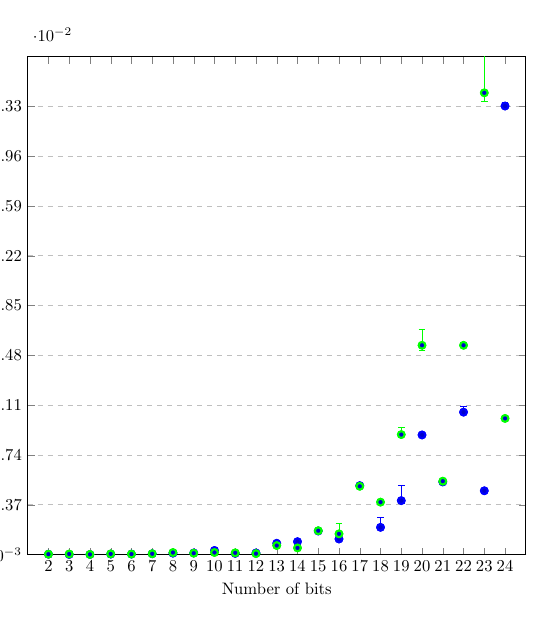
\begin{tikzpicture}[scale=0.6, trim axis left, trim axis right]
\begin{axis}[
    width=1\textwidth,
    height=1\textwidth,
    xlabel={Number of bits},
    ylabel={Time taken (s)},
    xmin=1.0, xmax=25.0,
    ymin=1.5e-05, ymax=0.037,
    xticklabels={2, 3, 4, 5, 6, 7, 8, 9, 10, 11, 12, 13, 14, 15, 16, 17, 18, 19, 20, 21, 22, 23, 24},
    xtick={2, 3, 4, 5, 6, 7, 8, 9, 10, 11, 12, 13, 14, 15, 16, 17, 18, 19, 20, 21, 22, 23, 24},
    ytick={0.0000150000000000000, 0.00371350000000000, 0.00741200000000000, 0.0111105000000000, 0.0148090000000000, 0.0185075000000000, 0.0222060000000000, 0.0259045000000000, 0.0296030000000000, 0.0333015000000000},
    ymajorgrids=true,
    grid style=dashed,
]

%%%%
%% Default
%%%%

\addplot+[
    blue,
    very thick,
    forget plot,
    only marks
    ]
    plot[
    very thick,
    error bars/.cd,
    y dir=plus,
    y explicit
    ]
    table[x=x,y=y,y error expr=\thisrow{y-max}] {
    x    y    y-max
    24	0.0333192	0.0002938
20	0.0088994	0.0001436
21	0.005411	0.000181
22	0.0105919	0.0004511
23	0.0047538	6.42e-05
3	2.51e-05	8.19e-05
2	4.4e-05	0.000184
5	5.34e-05	7.86e-05
4	2.6e-05	3e-06
7	7.86e-05	7.94e-05
6	5.36e-05	7.84e-05
9	0.0001385	1.25e-05
8	0.0001217	7.63e-05
11	0.0001041	7.39e-05
10	0.0003235	7.35e-05
13	0.0008575	6.35e-05
12	0.0001385	7.65e-05
15	0.001766	2.1e-05
14	0.0009775	4.95e-05
17	0.0051386	5.84e-05
16	0.0011735	7.25e-05
19	0.0040232	0.0011198
18	0.0020383	0.0007457

    };

\addplot+[
    blue,
    very thick,
    forget plot,
    only marks
    ]
    plot[
    very thick,
    error bars/.cd,
    y dir=plus,
    y explicit
    ]
    table[x=x,y=y,y error expr=\thisrow{y-min}] {
    x    y    y-min
    24	0.0333192	-0.0001732
20	0.0088994	-8.24e-05
21	0.005411	-4.2e-05
22	0.0105919	-0.0001079
23	0.0047538	-2.78e-05
3	2.51e-05	-1.01e-05
2	4.4e-05	-2.4e-05
5	5.34e-05	-9.4e-06
4	2.6e-05	-1e-06
7	7.86e-05	-9.6e-06
6	5.36e-05	-9.6e-06
9	0.0001385	-2.5e-06
8	0.0001217	-1.07e-05
11	0.0001041	-1.11e-05
10	0.0003235	-1.25e-05
13	0.0008575	-1.25e-05
12	0.0001385	-9.5e-06
15	0.001766	-1.4e-05
14	0.0009775	-2.05e-05
17	0.0051386	-3.26e-05
16	0.0011735	-1.65e-05
19	0.0040232	-0.0001992
18	0.0020383	-0.0001203

    };
    
%%%%
%% SQRT
%%%%%

\addplot+[
    green,
    very thick,
    forget plot,
    only marks
    ]
    plot[
    very thick,
    error bars/.cd,
    y dir=plus,
    y explicit
    ]
    table[x=x,y=y,y error expr=\thisrow{y-max}] {
    x    y    y-max
    24	0.0101261	0.0001099
20	0.0155554	0.0012086
21	0.005468	8.6e-05
22	0.0155544	0.0002216
23	0.0342993	0.0031447
3	6.19e-05	8.31e-05
2	4.65e-05	0.0002275
5	6.82e-05	7.58e-05
4	3.02e-05	8.18e-05
7	7.96e-05	7.84e-05
6	5.46e-05	7.74e-05
9	0.0001187	7.33e-05
8	0.0001696	8.64e-05
11	0.0001458	7.52e-05
10	0.0001704	7.56e-05
13	0.0006876	8.24e-05
12	8.72e-05	7.48e-05
15	0.0017901	7.59e-05
14	0.0005122	8.28e-05
17	0.0050859	0.0001041
16	0.0015563	0.0007857
19	0.0089271	0.0005279
18	0.0039111	7.89e-05

    };

\addplot+[
    green,
    very thick,
    forget plot,
    only marks
    ]
    plot[
    very thick,
    error bars/.cd,
    y dir=plus,
    y explicit
    ]
    table[x=x,y=y,y error expr=\thisrow{y-min}] {
    x    y    y-min
    24	0.0101261	-0.0001051
20	0.0155554	-0.0003584
21	0.005468	-6.5e-05
22	0.0155544	-9.04e-05
23	0.0342993	-0.0006093
3	6.19e-05	-1.29e-05
2	4.65e-05	-2.65e-05
5	6.82e-05	-1.02e-05
4	3.02e-05	-9.2e-06
7	7.96e-05	-9.6e-06
6	5.46e-05	-8.6e-06
9	0.0001187	-1.17e-05
8	0.0001696	-1.06e-05
11	0.0001458	-8.8e-06
10	0.0001704	-9.4e-06
13	0.0006876	-1.16e-05
12	8.72e-05	-9.2e-06
15	0.0017901	-3.71e-05
14	0.0005122	-1.12e-05
17	0.0050859	-5.19e-05
16	0.0015563	-0.0001093
19	0.0089271	-0.0001331
18	0.0039111	-2.01e-05

    };

\end{axis}
\end{tikzpicture}


    \vspace{-0.3cm}
    \caption{The two tested start values}\label{fig:pollardsStart}
\end{figure}

For factors of lower bit count, $x_0=y_0=2$ (shown in blue) and $x_0=y_0=\ceil[\big]{\sqrt{n}}$ (shown in green) seem to perform equally well. For larger bit count, blue seem to perform better.

It should be noted that only about half of the available numbers to test were tested in the above benchmarks.

\subsection{Two Factors}


\begin{figure}[H]
\centering
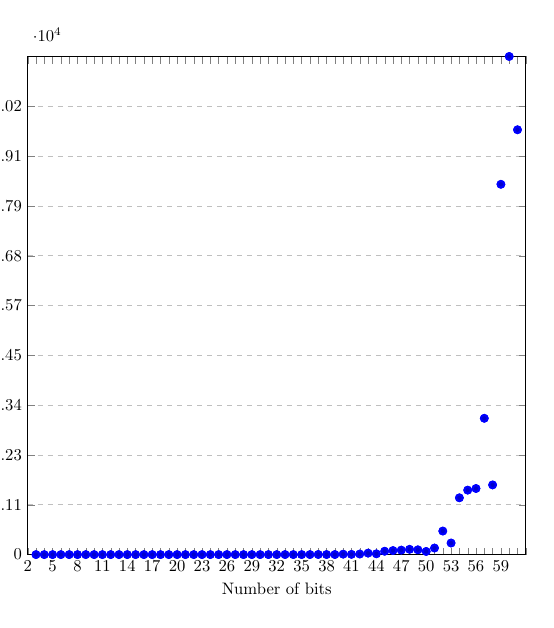
\begin{tikzpicture}[scale=0.6, trim axis left, trim axis right]
\begin{axis}[
    width=1\textwidth,
    height=1\textwidth,
    xlabel={Number of bits},
    ylabel={Time taken (s)},
    xmin=1.0, xmax=61.0,
    ymin=1.5e-05, ymax=11321.818036,
    xticklabels={2, , , 5, , , 8, , , 11, , , 14, , , 17, , , 20, , , 23, , , 26, , , 29, , , 32, , , 35, , , 38, , , 41, , , 44, , , 47, , , 50, , , 53, , , 56, , , 59, },
    xtick={1, 2, 3, 4, 5, 6, 7, 8, 9, 10, 11, 12, 13, 14, 15, 16, 17, 18, 19, 20, 21, 22, 23, 24, 25, 26, 27, 28, 29, 30, 31, 32, 33, 34, 35, 36, 37, 38, 39, 40, 41, 42, 43, 44, 45, 46, 47, 48, 49, 50, 51, 52, 53, 54, 55, 56, 57, 58, 59, 60, 61},
    ytick={1.5e-05, 1132.1818171, 2264.3636192, 3396.5454213, 4528.7272234, 5660.9090255, 6793.0908276, 7925.2726297, 9057.4544318, 10189.6362339},
    ymajorgrids=true,
    grid style=dashed,
]

\addplot+[
    blue,
    very thick,
    forget plot,
    only marks
    ]
    plot[
    very thick,
    error bars/.cd,
    y dir=plus,
    y explicit
    ]
    table[x=x,y=y,y error expr=\thisrow{y-max}] {
    x    y    y-max
    30	0.161975	0.0
37	1.311169	0.0
48	108.761925	0.0
45	91.73595	0.0
43	17.83201	0.0
60	9655.960219	0.0
35	0.926861	0.0
32	0.849543	0.0
24	0.0333192	0.0002938
25	0.064159	0.0
26	0.043284	0.0
27	0.035551	0.0
20	0.0088994	0.0001436
21	0.005411	0.000181
22	0.0105919	0.0004511
23	0.0047538	6.42e-05
46	101.69973	0.0
47	120.210968	0.0
44	76.279777	0.0
42	33.154922	0.0
28	0.084783	0.0
29	0.191224	0.0
40	5.029217	0.0
41	12.837914	0.0
3	2.51e-05	8.19e-05
2	4.4e-05	0.000184
5	5.34e-05	7.86e-05
4	2.6e-05	3e-06
7	7.86e-05	7.94e-05
6	5.36e-05	7.84e-05
9	0.0001385	1.25e-05
8	0.0001217	7.63e-05
49	71.629152	0.0
33	0.439183	0.0
39	10.141911	0.0
34	0.310229	0.0
38	1.542419	0.0
15	0.001766	2.1e-05
14	0.0009775	4.95e-05
11	0.0001041	7.39e-05
10	0.0003235	7.35e-05
13	0.0008575	6.35e-05
12	0.0001385	7.65e-05
59	11321.818036	0.0
58	8416.254496	0.0
17	0.0051386	5.84e-05
16	0.0011735	7.25e-05
19	0.0040232	0.0011198
18	0.0020383	0.0007457
57	1583.803046	0.0
56	3097.92530925	7.93628075
51	535.1181588	2.1523022
36	2.69102	0.0
53	1290.4938745	3.7281665
52	263.3708634	1.0185996
55	1502.6130217	6.4900103
54	1465.386043	5.744853
31	0.078828	0.0
50	149.559654	0.0

    };

\addplot+[
    blue,
    very thick,
    forget plot,
    only marks
    ]
    plot[
    very thick,
    error bars/.cd,
    y dir=plus,
    y explicit
    ]
    table[x=x,y=y,y error expr=\thisrow{y-min}] {
    x    y    y-min
    30	0.161975	0.0
37	1.311169	0.0
48	108.761925	0.0
45	91.73595	0.0
43	17.83201	0.0
60	9655.960219	0.0
35	0.926861	0.0
32	0.849543	0.0
24	0.0333192	-0.0001732
25	0.064159	0.0
26	0.043284	0.0
27	0.035551	0.0
20	0.0088994	-8.24e-05
21	0.005411	-4.2e-05
22	0.0105919	-0.0001079
23	0.0047538	-2.78e-05
46	101.69973	0.0
47	120.210968	0.0
44	76.279777	0.0
42	33.154922	0.0
28	0.084783	0.0
29	0.191224	0.0
40	5.029217	0.0
41	12.837914	0.0
3	2.51e-05	-1.01e-05
2	4.4e-05	-2.4e-05
5	5.34e-05	-9.4e-06
4	2.6e-05	-1e-06
7	7.86e-05	-9.6e-06
6	5.36e-05	-9.6e-06
9	0.0001385	-2.5e-06
8	0.0001217	-1.07e-05
49	71.629152	0.0
33	0.439183	0.0
39	10.141911	0.0
34	0.310229	0.0
38	1.542419	0.0
15	0.001766	-1.4e-05
14	0.0009775	-2.05e-05
11	0.0001041	-1.11e-05
10	0.0003235	-1.25e-05
13	0.0008575	-1.25e-05
12	0.0001385	-9.5e-06
59	11321.818036	0.0
58	8416.254496	0.0
17	0.0051386	-3.26e-05
16	0.0011735	-1.65e-05
19	0.0040232	-0.0001992
18	0.0020383	-0.0001203
57	1583.803046	0.0
56	3097.92530925	-14.63882725
51	535.1181588	-2.0290468
36	2.69102	0.0
53	1290.4938745	-2.0932065
52	263.3708634	-2.5243514
55	1502.6130217	-4.5145147
54	1465.386043	-5.111975
31	0.078828	0.0
50	149.559654	0.0

    };

\end{axis}
\end{tikzpicture}
\vspace{-0.3cm}
\caption{Factors between 2 and 60 bits}\label{fig:PollardsRhoAlgorithmGrowingprimesbits260}
\end{figure}

In figure \ref{fig:PollardsRhoAlgorithmGrowingprimesbits260} all tested numbers can be seen. To better interpret the results, plots showing lesser ranges of tests can be found in the appendix in figure \ref{fig:PollardsRhoAlgorithmGrowingprimesbits250}, \ref{fig:PollardsRhoAlgorithmGrowingprimesbits240}, \ref{fig:PollardsRhoAlgorithmGrowingprimesbits230} and \ref{fig:PollardsRhoAlgorithmGrowingprimesbits220}, respectively.

\subsection{Multiple Factors}\label{PollardsMultipleFactors}

Below are seven groups of plots determining the performance of Pollard's Rho Algorithm. A lower value refers to lower time taken, which is considered better. The figures shown will be in ascending order within their respective class.


\begin{figure}[H]
\centering
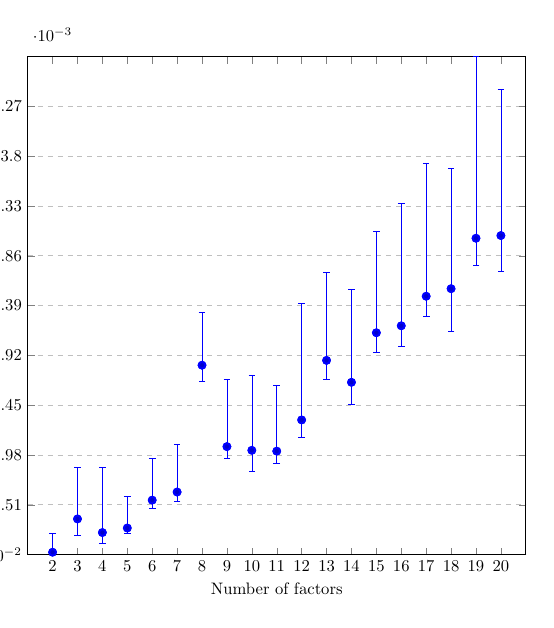
\begin{tikzpicture}[scale=0.6, trim axis left, trim axis right]
\begin{axis}[
    width=1\textwidth,
    height=1\textwidth,
    xlabel={Number of factors},
    ylabel={Time taken (s)},
    xmin=1.0, xmax=21.0,
    ymin=4e-05, ymax=0.004735,
    xticklabels={2, 3, 4, 5, 6, 7, 8, 9, 10, 11, 12, 13, 14, 15, 16, 17, 18, 19, 20},
    xtick={2, 3, 4, 5, 6, 7, 8, 9, 10, 11, 12, 13, 14, 15, 16, 17, 18, 19, 20},
    ytick={4e-05, 0.0005095, 0.000979, 0.0014485, 0.001918, 0.0023875, 0.002857, 0.0033265, 0.003796, 0.0042655},
    ymajorgrids=true,
    grid style=dashed,
]

\addplot+[
    blue,
    very thick,
    forget plot,
    only marks
    ]
    plot[
    very thick,
    error bars/.cd,
    y dir=plus,
    y explicit
    ]
    table[x=x,y=y,y error expr=\thisrow{y-max}] {
    x    y    y-max
    11	0.0010151	0.0006189
10	0.0010229	0.0007071
13	0.0018704	0.0008266
12	0.00130915	0.00109585
15	0.00213095	0.00095605
14	0.00166385	0.00087315
17	0.00247505	0.00125595
16	0.00219655	0.00115145
19	0.0030217	0.0017133
18	0.0025462	0.0011298
20	0.003047	0.001376
3	0.00037625	0.00049075
2	6.235e-05	0.00018165
5	0.0002906	0.0002984
4	0.00024795	0.00061905
7	0.0006298	0.0004522
6	0.00055335	0.00039265
9	0.0010578	0.0006302
8	0.0018249	0.0005031

    };

\addplot+[
    blue,
    very thick,
    forget plot,
    only marks
    ]
    plot[
    very thick,
    error bars/.cd,
    y dir=plus,
    y explicit
    ]
    table[x=x,y=y,y error expr=\thisrow{y-min}] {
    x    y    y-min
    11	0.0010151	-0.0001121
10	0.0010229	-0.0001999
13	0.0018704	-0.0001764
12	0.00130915	-0.00016515
15	0.00213095	-0.00018795
14	0.00166385	-0.00020785
17	0.00247505	-0.00018905
16	0.00219655	-0.00019455
19	0.0030217	-0.0002577
18	0.0025462	-0.0004062
20	0.003047	-0.000337
3	0.00037625	-0.00015725
2	6.235e-05	-2.235e-05
5	0.0002906	-4.76e-05
4	0.00024795	-0.00010295
7	0.0006298	-8.58e-05
6	0.00055335	-7.335e-05
9	0.0010578	-0.0001088
8	0.0018249	-0.0001509

    };

\end{axis}
\end{tikzpicture}
\vspace{-0.3cm}
\caption{Small primes}\label{fig:PollardsRhoAlgorithmsmallprimesfactors}
\end{figure}



From the figure \ref{fig:PollardsRhoAlgorithmsmallprimesfactors} one can tell that the algorithm does not seem to perform equally well every time it is tested on the same number. Looking closely and with an open eye, there seem to be some correlation with every two data points. The reason for this correlation is not known. All in all, an approximate curve would have to be steeper than a linear fit. 


\begin{figure}[H]
\centering
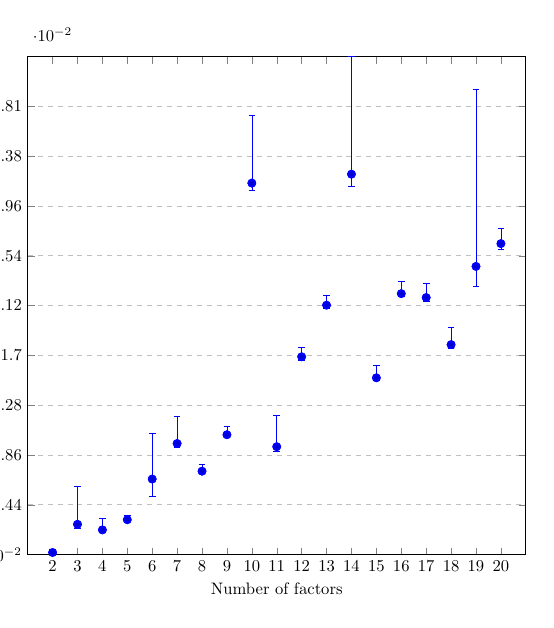
\begin{tikzpicture}[scale=0.6, trim axis left, trim axis right]
\begin{axis}[
    width=1\textwidth,
    height=1\textwidth,
    xlabel={Number of factors},
    ylabel={Time taken (s)},
    xmin=1.0, xmax=21.0,
    ymin=0.000164, ymax=0.042271,
    xticklabels={2, 3, 4, 5, 6, 7, 8, 9, 10, 11, 12, 13, 14, 15, 16, 17, 18, 19, 20},
    xtick={2, 3, 4, 5, 6, 7, 8, 9, 10, 11, 12, 13, 14, 15, 16, 17, 18, 19, 20},
    ytick={0.000164, 0.0043747, 0.0085854, 0.0127961, 0.0170068, 0.0212175, 0.0254282, 0.0296389, 0.0338496, 0.0380603},
    ymajorgrids=true,
    grid style=dashed,
]

\addplot+[
    blue,
    very thick,
    forget plot,
    only marks
    ]
    plot[
    very thick,
    error bars/.cd,
    y dir=plus,
    y explicit
    ]
    table[x=x,y=y,y error expr=\thisrow{y-max}] {
    x    y    y-max
    11	0.00928585	0.00266415
10	0.0315662	0.0056918
13	0.02124855	0.00085645
12	0.0168851	0.0008109
15	0.01510675	0.00105825
14	0.0323219	0.0099491
17	0.0218915	0.0012355
16	0.02222265	0.00104635
19	0.02452565	0.01497135
18	0.0179121	0.0015029
20	0.0264522	0.0012788
3	0.00272305	0.00323395
2	0.00034315	0.00026385
5	0.00311105	0.00034895
4	0.0022519	0.0009901
7	0.00955625	0.00228975
6	0.0065518	0.0038972
9	0.010298	0.000692
8	0.00721455	0.00057345

    };

\addplot+[
    blue,
    very thick,
    forget plot,
    only marks
    ]
    plot[
    very thick,
    error bars/.cd,
    y dir=plus,
    y explicit
    ]
    table[x=x,y=y,y error expr=\thisrow{y-min}] {
    x    y    y-min
    11	0.00928585	-0.00035485
10	0.0315662	-0.0005842
13	0.02124855	-0.00028655
12	0.0168851	-0.0002761
15	0.01510675	-0.00025375
14	0.0323219	-0.0009959
17	0.0218915	-0.0003015
16	0.02222265	-0.00025265
19	0.02452565	-0.00165265
18	0.0179121	-0.0002801
20	0.0264522	-0.0004572
3	0.00272305	-0.00034205
2	0.00034315	-0.00017915
5	0.00311105	-8.505e-05
4	0.0022519	-0.0001279
7	0.00955625	-0.00032025
6	0.0065518	-0.0014818
9	0.010298	-0.000128
8	0.00721455	-0.00015755

    };

\end{axis}
\end{tikzpicture}
\vspace{-0.3cm}
\caption{Medium primes}\label{fig:PollardsRhoAlgorithmmediumprimesfactors}
\end{figure}



The figure \ref{fig:PollardsRhoAlgorithmmediumprimesfactors} shows signs of even more irregularity than figure \ref{fig:PollardsRhoAlgorithmsmallprimesfactors}. The average span between the lowest time taken and the maximum time taken is lower than the first figure. The slight correlation with every two data points seen in the previous figure seem to be lost. Interestingly the first data point, for two factors, seem to take about the same time as the first number tested for small primes.


\begin{figure}[H]
\centering
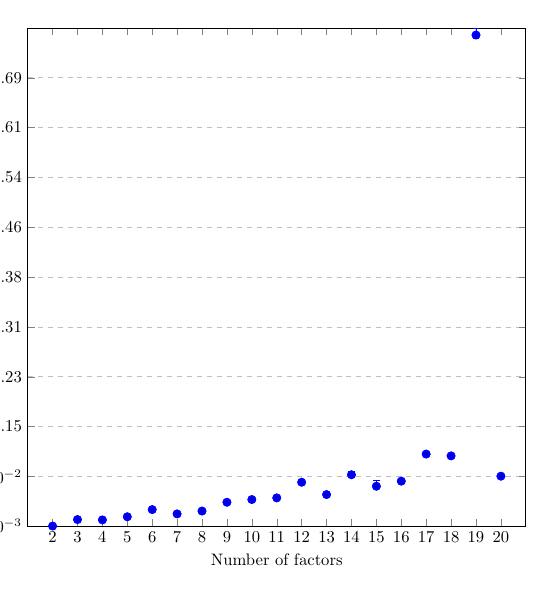
\begin{tikzpicture}[scale=0.6, trim axis left, trim axis right]
\begin{axis}[
    width=1\textwidth,
    height=1\textwidth,
    xlabel={Number of factors},
    ylabel={Time taken (s)},
    xmin=1.0, xmax=21.0,
    ymin=0.001207, ymax=0.764686,
    xticklabels={2, 3, 4, 5, 6, 7, 8, 9, 10, 11, 12, 13, 14, 15, 16, 17, 18, 19, 20},
    xtick={2, 3, 4, 5, 6, 7, 8, 9, 10, 11, 12, 13, 14, 15, 16, 17, 18, 19, 20},
    ytick={0.001207, 0.0775549, 0.1539028, 0.2302507, 0.3065986, 0.3829465, 0.4592944, 0.5356423, 0.6119902, 0.6883381},
    ymajorgrids=true,
    grid style=dashed,
]

\addplot+[
    blue,
    very thick,
    forget plot,
    only marks
    ]
    plot[
    very thick,
    error bars/.cd,
    y dir=plus,
    y explicit
    ]
    table[x=x,y=y,y error expr=\thisrow{y-max}] {
    x    y    y-max
    11	0.044532	0.000897
10	0.0420184	0.0008156
13	0.04962435	0.00068165
12	0.06852925	0.00206375
15	0.0623668	0.0097712
14	0.08000975	0.00501025
17	0.1116782	0.0008588
16	0.0702068	0.0029382
19	0.753904533333	0.0107814666667
18	0.1089075	0.0012035
20	0.077806	0.001313
3	0.01134375	0.00099925
2	0.0013532	0.0009598
5	0.01559695	0.00158205
4	0.010776	0.001642
7	0.02000145	0.00049055
6	0.0265808	0.0005602
9	0.03781025	0.00062275
8	0.0243461	0.0005969

    };

\addplot+[
    blue,
    very thick,
    forget plot,
    only marks
    ]
    plot[
    very thick,
    error bars/.cd,
    y dir=plus,
    y explicit
    ]
    table[x=x,y=y,y error expr=\thisrow{y-min}] {
    x    y    y-min
    11	0.044532	-0.000456
10	0.0420184	-0.0002514
13	0.04962435	-0.00038535
12	0.06852925	-0.00046625
15	0.0623668	-0.0017908
14	0.08000975	-0.00127275
17	0.1116782	-0.0009772
16	0.0702068	-0.0005448
19	0.753904533333	-0.00489953333333
18	0.1089075	-0.0008165
20	0.077806	-0.000883
3	0.01134375	-0.00019875
2	0.0013532	-0.0001462
5	0.01559695	-0.00025295
4	0.010776	-0.00021
7	0.02000145	-0.00018445
6	0.0265808	-0.0002378
9	0.03781025	-0.00051125
8	0.0243461	-0.0001791

    };

\end{axis}
\end{tikzpicture}
\vspace{-0.3cm}
\caption{Large primes}\label{fig:PollardsRhoAlgorithmlargeprimesfactors}
\end{figure}



The figure \ref{fig:PollardsRhoAlgorithmLargerprimesfactors} show one extreme point. Removing the point show a second figure show below in figure \ref{fig:PollardsRhoAlgorithmlargeprimesfactors2}.


\begin{figure}[H]
\centering
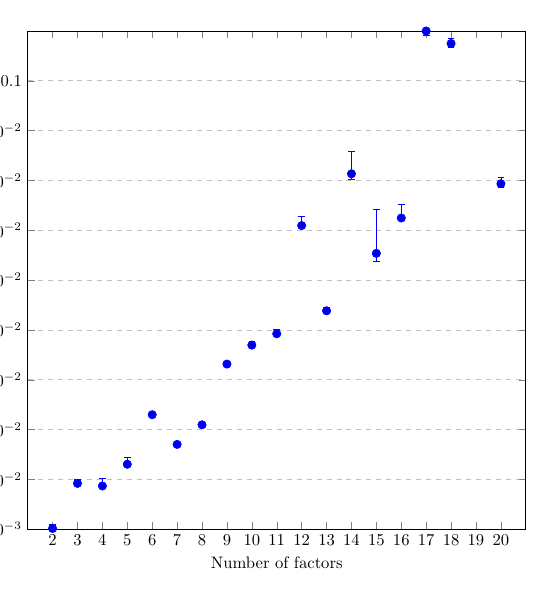
\begin{tikzpicture}[scale=0.6, trim axis left, trim axis right]
\begin{axis}[
    width=1\textwidth,
    height=1\textwidth,
    xlabel={Number of factors},
    ylabel={Time taken (s)},
    xmin=1.0, xmax=21.0,
    ymin=0.001207, ymax=0.1116782,
    xticklabels={2, 3, 4, 5, 6, 7, 8, 9, 10, 11, 12, 13, 14, 15, 16, 17, 18, 19, 20},
    xtick={2, 3, 4, 5, 6, 7, 8, 9, 10, 11, 12, 13, 14, 15, 16, 17, 18, 19, 20},
    ytick={0.00120700000000000, 0.0122541200000000, 0.0233012400000000, 0.0343483600000000, 0.0453954800000000, 0.0564426000000000, 0.0674897200000000, 0.0785368400000000, 0.0895839600000000, 0.100631080000000},
    ymajorgrids=true,
    grid style=dashed,
]

\addplot+[
    blue,
    very thick,
    forget plot,
    only marks
    ]
    plot[
    very thick,
    error bars/.cd,
    y dir=plus,
    y explicit
    ]
    table[x=x,y=y,y error expr=\thisrow{y-max}] {
    x    y    y-max
    11	0.044532	0.000897
10	0.0420184	0.0008156
13	0.04962435	0.00068165
12	0.06852925	0.00206375
15	0.0623668	0.0097712
14	0.08000975	0.00501025
17	0.1116782	0.0008588
16	0.0702068	0.0029382
18	0.1089075	0.0012035
20	0.077806	0.001313
3	0.01134375	0.00099925
2	0.0013532	0.0009598
5	0.01559695	0.00158205
4	0.010776	0.001642
7	0.02000145	0.00049055
6	0.0265808	0.0005602
9	0.03781025	0.00062275
8	0.0243461	0.0005969

    };

\addplot+[
    blue,
    very thick,
    forget plot,
    only marks
    ]
    plot[
    very thick,
    error bars/.cd,
    y dir=plus,
    y explicit
    ]
    table[x=x,y=y,y error expr=\thisrow{y-min}] {
    x    y    y-min
    11	0.044532	-0.000456
10	0.0420184	-0.0002514
13	0.04962435	-0.00038535
12	0.06852925	-0.00046625
15	0.0623668	-0.0017908
14	0.08000975	-0.00127275
17	0.1116782	-0.0009772
16	0.0702068	-0.0005448
18	0.1089075	-0.0008165
20	0.077806	-0.000883
3	0.01134375	-0.00019875
2	0.0013532	-0.0001462
5	0.01559695	-0.00025295
4	0.010776	-0.00021
7	0.02000145	-0.00018445
6	0.0265808	-0.0002378
9	0.03781025	-0.00051125
8	0.0243461	-0.0001791

    };

\end{axis}
\end{tikzpicture}
\vspace{-0.3cm}
\caption{Large primes, closer window}\label{fig:PollardsRhoAlgorithmlargeprimesfactors2}
\end{figure}



The figure shows an average span between the maximum time taken and the minimum time taken to factorize a number is about the same as shown for medium sized prime factors in figure \ref{fig:PollardsRhoAlgorithmmediumprimesfactors}.


\begin{figure}[H]
\centering
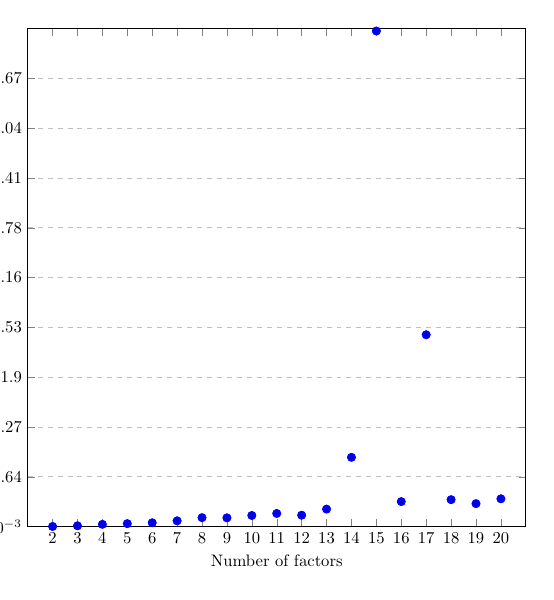
\begin{tikzpicture}[scale=0.6, trim axis left, trim axis right]
\begin{axis}[
    width=1\textwidth,
    height=1\textwidth,
    xlabel={Number of factors},
    ylabel={Time taken (s)},
    xmin=1.0, xmax=21.0,
    ymin=0.005904, ymax=6.304297,
    xticklabels={2, 3, 4, 5, 6, 7, 8, 9, 10, 11, 12, 13, 14, 15, 16, 17, 18, 19, 20},
    xtick={2, 3, 4, 5, 6, 7, 8, 9, 10, 11, 12, 13, 14, 15, 16, 17, 18, 19, 20},
    ytick={0.005904, 0.6357433, 1.2655826, 1.8954219, 2.5252612, 3.1551005, 3.7849398, 4.4147791, 5.0446184, 5.6744577},
    ymajorgrids=true,
    grid style=dashed,
]

\addplot+[
    blue,
    very thick,
    forget plot,
    only marks
    ]
    plot[
    very thick,
    error bars/.cd,
    y dir=plus,
    y explicit
    ]
    table[x=x,y=y,y error expr=\thisrow{y-max}] {
    x    y    y-max
    11	0.1717384	0.0004546
10	0.1462144	0.0009446
13	0.2267711	0.0005079
12	0.1498062	0.0004768
15	6.2717134	0.0325836
14	0.8811528	0.0257212
17	2.4309682	0.0055518
16	0.3213873	0.0009757
19	0.29544	0.000853
18	0.3459382	0.0017908
20	0.3569991	0.0021129
3	0.0156157	0.0011213
2	0.0070451	0.0076699
5	0.0429597	0.0013313
4	0.0338899	0.0082351
7	0.078487	0.000818
6	0.0539048	0.0017162
9	0.1164037	0.0146073
8	0.1185742	0.0009988

    };

\addplot+[
    blue,
    very thick,
    forget plot,
    only marks
    ]
    plot[
    very thick,
    error bars/.cd,
    y dir=plus,
    y explicit
    ]
    table[x=x,y=y,y error expr=\thisrow{y-min}] {
    x    y    y-min
    11	0.1717384	-0.0007464
10	0.1462144	-0.0006734
13	0.2267711	-0.0005571
12	0.1498062	-0.0005382
15	6.2717134	-0.0294054
14	0.8811528	-0.0081398
17	2.4309682	-0.0127442
16	0.3213873	-0.0008923
19	0.29544	-0.001212
18	0.3459382	-0.0019042
20	0.3569991	-0.0013671
3	0.0156157	-0.0002927
2	0.0070451	-0.0011411
5	0.0429597	-0.0003927
4	0.0338899	-0.0011799
7	0.078487	-0.000379
6	0.0539048	-0.0004508
9	0.1164037	-0.0021017
8	0.1185742	-0.0009572

    };

\end{axis}
\end{tikzpicture}
\vspace{-0.3cm}
\caption{Larger primes}\label{fig:PollardsRhoAlgorithmLargerprimesfactors}
\end{figure}



When factorizing even larger numbers consisting of up to $20$ prime factors, Pollard's Rho Algorithm seem to perform under half a second for most numbers. By removing the highest three data points, the next figure was made to more clearly show the differences between the data points.


\begin{figure}[H]
\centering
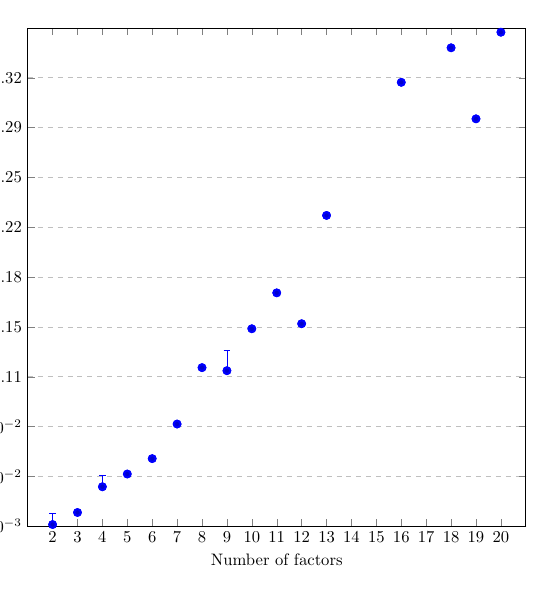
\begin{tikzpicture}[scale=0.6, trim axis left, trim axis right]
\begin{axis}[
    width=1\textwidth,
    height=1\textwidth,
    xlabel={Number of factors},
    ylabel={Time taken (s)},
    xmin=1.0, xmax=21.0,
    ymin=0.005904, ymax=0.36,
    xticklabels={2, 3, 4, 5, 6, 7, 8, 9, 10, 11, 12, 13, 14, 15, 16, 17, 18, 19, 20},
    xtick={2, 3, 4, 5, 6, 7, 8, 9, 10, 11, 12, 13, 14, 15, 16, 17, 18, 19, 20},
    ytick={0.00590400000000000, 0.0413136000000000, 0.0767232000000000, 0.112132800000000, 0.147542400000000, 0.182952000000000, 0.218361600000000, 0.253771200000000, 0.289180800000000, 0.324590400000000},
    ymajorgrids=true,
    grid style=dashed,
]

\addplot+[
    blue,
    very thick,
    forget plot,
    only marks
    ]
    plot[
    very thick,
    error bars/.cd,
    y dir=plus,
    y explicit
    ]
    table[x=x,y=y,y error expr=\thisrow{y-max}] {
    x    y    y-max
    11	0.1717384	0.0004546
10	0.1462144	0.0009446
13	0.2267711	0.0005079
12	0.1498062	0.0004768
16	0.3213873	0.0009757
19	0.29544	0.000853
18	0.3459382	0.0017908
20	0.3569991	0.0021129
3	0.0156157	0.0011213
2	0.0070451	0.0076699
5	0.0429597	0.0013313
4	0.0338899	0.0082351
7	0.078487	0.000818
6	0.0539048	0.0017162
9	0.1164037	0.0146073
8	0.1185742	0.0009988

    };

\addplot+[
    blue,
    very thick,
    forget plot,
    only marks
    ]
    plot[
    very thick,
    error bars/.cd,
    y dir=plus,
    y explicit
    ]
    table[x=x,y=y,y error expr=\thisrow{y-min}] {
    x    y    y-min
    11	0.1717384	-0.0007464
10	0.1462144	-0.0006734
13	0.2267711	-0.0005571
12	0.1498062	-0.0005382
16	0.3213873	-0.0008923
19	0.29544	-0.001212
18	0.3459382	-0.0019042
20	0.3569991	-0.0013671
3	0.0156157	-0.0002927
2	0.0070451	-0.0011411
5	0.0429597	-0.0003927
4	0.0338899	-0.0011799
7	0.078487	-0.000379
6	0.0539048	-0.0004508
9	0.1164037	-0.0021017
8	0.1185742	-0.0009572

    };

\end{axis}
\end{tikzpicture}
\vspace{-0.3cm}
\caption{Larger primes, closer window}\label{fig:PollardsRhoAlgorithmLargerprimesfactors2}
\end{figure}


\begin{figure}[H]
\centering
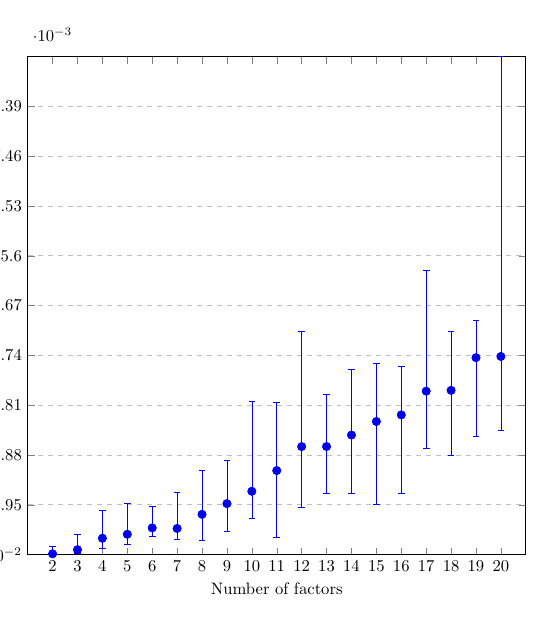
\begin{tikzpicture}[scale=0.6, trim axis left, trim axis right]
\begin{axis}[
    width=1\textwidth,
    height=1\textwidth,
    xlabel={Number of factors},
    ylabel={Time taken (s)},
    xmin=1.0, xmax=21.0,
    ymin=1.9e-05, ymax=0.009317,
    xticklabels={2, 3, 4, 5, 6, 7, 8, 9, 10, 11, 12, 13, 14, 15, 16, 17, 18, 19, 20},
    xtick={2, 3, 4, 5, 6, 7, 8, 9, 10, 11, 12, 13, 14, 15, 16, 17, 18, 19, 20},
    ytick={1.9e-05, 0.0009488, 0.0018786, 0.0028084, 0.0037382, 0.004668, 0.0055978, 0.0065276, 0.0074574, 0.0083872},
    ymajorgrids=true,
    grid style=dashed,
]

\addplot+[
    blue,
    very thick,
    forget plot,
    only marks
    ]
    plot[
    very thick,
    error bars/.cd,
    y dir=plus,
    y explicit
    ]
    table[x=x,y=y,y error expr=\thisrow{y-max}] {
    x    y    y-max
    11	0.0015875125	0.0012754875
10	0.0012010125	0.0016709875
13	0.002036125	0.000979875
12	0.0020351	0.0021599
15	0.002503125	0.001089875
14	0.002250675	0.001235325
17	0.0030697125	0.0022602875
16	0.0026267125	0.0009122875
19	0.0036951125	0.0007028875
18	0.0030848125	0.0010931875
20	0.0037176625	0.0055993375
3	0.0001103875	0.0002796125
2	3.39e-05	0.0001341
5	0.00039845	0.00058655
4	0.0003240375	0.0005159625
7	0.0005071375	0.0006688625
6	0.000517675	0.000393325
9	0.00097005	0.00080495
8	0.0007702875	0.0008277125

    };

\addplot+[
    blue,
    very thick,
    forget plot,
    only marks
    ]
    plot[
    very thick,
    error bars/.cd,
    y dir=plus,
    y explicit
    ]
    table[x=x,y=y,y error expr=\thisrow{y-min}] {
    x    y    y-min
    11	0.0015875125	-0.0012555125
10	0.0012010125	-0.0005090125
13	0.002036125	-0.000870125
12	0.0020351	-0.0011361
15	0.002503125	-0.001550125
14	0.002250675	-0.001081675
17	0.0030697125	-0.0010707125
16	0.0026267125	-0.0014727125
19	0.0036951125	-0.0014611125
18	0.0030848125	-0.0012128125
20	0.0037176625	-0.0013776625
3	0.0001103875	-5.93875e-05
2	3.39e-05	-1.49e-05
5	0.00039845	-0.00018945
4	0.0003240375	-0.0001810375
7	0.0005071375	-0.0001991375
6	0.000517675	-0.000158675
9	0.00097005	-0.00051205
8	0.0007702875	-0.0004912875

    };

\end{axis}
\end{tikzpicture}
\vspace{-0.3cm}
\caption{Small primes, close primes}\label{fig:PollardsRhoAlgorithmSmallcloseprimesfactors}
\end{figure}



Figure \ref{fig:PollardsRhoAlgorithmSmallcloseprimesfactors} shows numbers consisting of small prime factors close to one another. The factorization time span is clearly higher than that of previous benchmarks. The highest time taken for small primes shown in figure \ref{fig:PollardsRhoAlgorithmsmallprimesfactors} is about the same as the highest time taken for small close primes, shown above.


\begin{figure}[H]
\centering
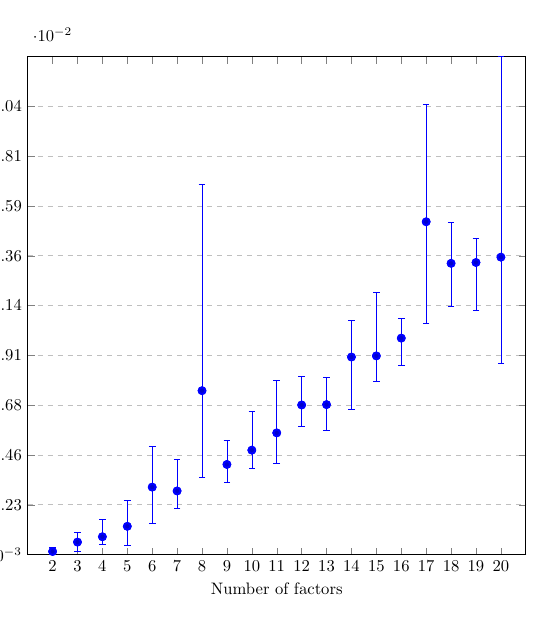
\begin{tikzpicture}[scale=0.6, trim axis left, trim axis right]
\begin{axis}[
    width=1\textwidth,
    height=1\textwidth,
    xlabel={Number of factors},
    ylabel={Time taken (s)},
    xmin=1.0, xmax=21.0,
    ymin=8.5e-05, ymax=0.022634,
    xticklabels={2, 3, 4, 5, 6, 7, 8, 9, 10, 11, 12, 13, 14, 15, 16, 17, 18, 19, 20},
    xtick={2, 3, 4, 5, 6, 7, 8, 9, 10, 11, 12, 13, 14, 15, 16, 17, 18, 19, 20},
    ytick={8.5e-05, 0.0023399, 0.0045948, 0.0068497, 0.0091046, 0.0113595, 0.0136144, 0.0158693, 0.0181242, 0.0203791},
    ymajorgrids=true,
    grid style=dashed,
]

\addplot+[
    blue,
    very thick,
    forget plot,
    only marks
    ]
    plot[
    very thick,
    error bars/.cd,
    y dir=plus,
    y explicit
    ]
    table[x=x,y=y,y error expr=\thisrow{y-max}] {
    x    y    y-max
    11	0.00559505	0.00237995
10	0.004813025	0.001770975
13	0.0068751	0.0012429
12	0.00685815	0.00130485
15	0.0090789	0.0028701
14	0.009028825	0.001659175
17	0.0151502	0.0053328
16	0.009884375	0.000903625
19	0.013307125	0.001105875
18	0.0132696	0.0018424
20	0.013549025	0.009084975
3	0.00065135	0.00041965
2	0.000225	0.000209
5	0.0013648	0.0011552
4	0.0008925	0.0007915
7	0.002965925	0.001411075
6	0.00314	0.001867
9	0.0041661	0.0011099
8	0.0075055	0.0093325

    };

\addplot+[
    blue,
    very thick,
    forget plot,
    only marks
    ]
    plot[
    very thick,
    error bars/.cd,
    y dir=plus,
    y explicit
    ]
    table[x=x,y=y,y error expr=\thisrow{y-min}] {
    x    y    y-min
    11	0.00559505	-0.00139505
10	0.004813025	-0.000838025
13	0.0068751	-0.0011631
12	0.00685815	-0.00095815
15	0.0090789	-0.0011349
14	0.009028825	-0.002366825
17	0.0151502	-0.0045782
16	0.009884375	-0.001215375
19	0.013307125	-0.002149125
18	0.0132696	-0.0019636
20	0.013549025	-0.004818025
3	0.00065135	-0.00040235
2	0.000225	-0.00014
5	0.0013648	-0.0008808
4	0.0008925	-0.0003565
7	0.002965925	-0.000789925
6	0.00314	-0.001623
9	0.0041661	-0.0007951
8	0.0075055	-0.0039055

    };

\end{axis}
\end{tikzpicture}
\vspace{-0.3cm}
\caption{Medium primes, close primes}\label{fig:PollardsRhoAlgorithmMediumcloseprimesfactors}
\end{figure}



Figure \ref{fig:PollardsRhoAlgorithmLargerprimesfactors} shows some extremes regarding factorization time spans.


\begin{figure}[H]
\centering
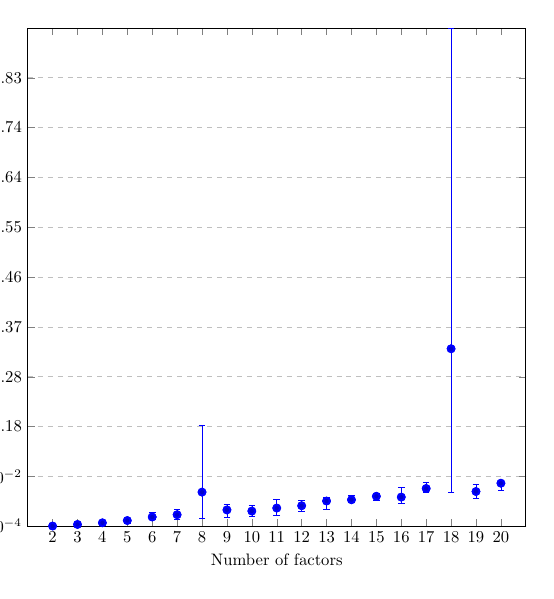
\begin{tikzpicture}[scale=0.6, trim axis left, trim axis right]
\begin{axis}[
    width=1\textwidth,
    height=1\textwidth,
    xlabel={Number of factors},
    ylabel={Time taken (s)},
    xmin=1.0, xmax=21.0,
    ymin=0.000512, ymax=0.920082,
    xticklabels={2, 3, 4, 5, 6, 7, 8, 9, 10, 11, 12, 13, 14, 15, 16, 17, 18, 19, 20},
    xtick={2, 3, 4, 5, 6, 7, 8, 9, 10, 11, 12, 13, 14, 15, 16, 17, 18, 19, 20},
    ytick={0.000512, 0.092469, 0.184426, 0.276383, 0.36834, 0.460297, 0.552254, 0.644211, 0.736168, 0.828125},
    ymajorgrids=true,
    grid style=dashed,
]

\addplot+[
    blue,
    very thick,
    forget plot,
    only marks
    ]
    plot[
    very thick,
    error bars/.cd,
    y dir=plus,
    y explicit
    ]
    table[x=x,y=y,y error expr=\thisrow{y-max}] {
    x    y    y-max
    11	0.0338855	0.0153075
10	0.02832205	0.01050395
13	0.046850025	0.007671975
12	0.03817985	0.01035515
15	0.055642425	0.005203575
14	0.049194325	0.008508675
17	0.0700452	0.0117008
16	0.0541392	0.0179668
19	0.064391975	0.013168025
18	0.3279611	0.5921209
20	0.07977395	0.00580105
3	0.003596125	0.001243875
2	0.000689725	0.000226275
5	0.010862175	0.004669825
4	0.00663995	0.00094305
7	0.02158775	0.01041225
6	0.017379675	0.008603325
9	0.030471175	0.010424825
8	0.063288925	0.123720075

    };

\addplot+[
    blue,
    very thick,
    forget plot,
    only marks
    ]
    plot[
    very thick,
    error bars/.cd,
    y dir=plus,
    y explicit
    ]
    table[x=x,y=y,y error expr=\thisrow{y-min}] {
    x    y    y-min
    11	0.0338855	-0.0129195
10	0.02832205	-0.00964605
13	0.046850025	-0.014557025
12	0.03817985	-0.01084385
15	0.055642425	-0.007311425
14	0.049194325	-0.005397325
17	0.0700452	-0.0067332
16	0.0541392	-0.0121832
19	0.064391975	-0.013276975
18	0.3279611	-0.2659121
20	0.07977395	-0.01245495
3	0.003596125	-0.000170125
2	0.000689725	-0.000177725
5	0.010862175	-0.004473175
4	0.00663995	-0.00098295
7	0.02158775	-0.00811975
6	0.017379675	-0.004444675
9	0.030471175	-0.013851175
8	0.063288925	-0.047473925

    };

\end{axis}
\end{tikzpicture}
\vspace{-0.3cm}
\caption{Large primes, close numbers}\label{fig:PollardsRhoAlgorithmLargecloseprimesfactors}
\end{figure}



Figure \ref{fig:PollardsRhoAlgorithmLargecloseprimesfactors} shows two extremes. Removing the data point reveals a second figure, \ref{fig:PollardsRhoAlgorithmLargecloseprimesfactors2} which more clearly depicts the change depending on number of factors.


\begin{figure}[H]
\centering
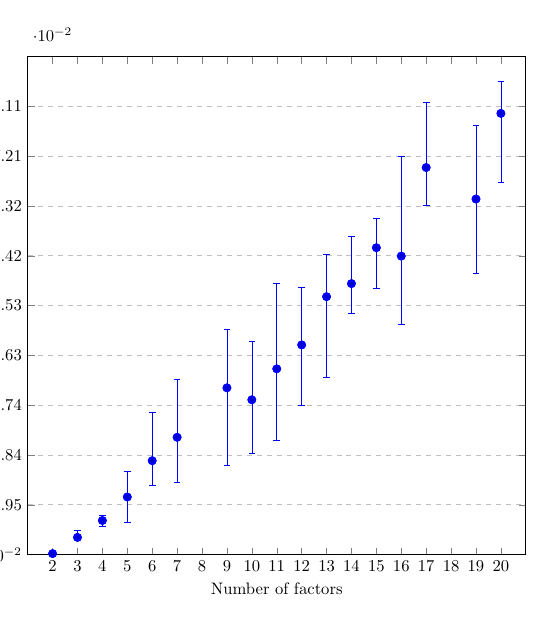
\begin{tikzpicture}[scale=0.6, trim axis left, trim axis right]
\begin{axis}[
    width=1\textwidth,
    height=1\textwidth,
    xlabel={Number of factors},
    ylabel={Time taken (s)},
    xmin=1.0, xmax=21.0,
    ymin=0.000512, ymax=0.09,
    xticklabels={2, 3, 4, 5, 6, 7, 8, 9, 10, 11, 12, 13, 14, 15, 16, 17, 18, 19, 20},
    xtick={2, 3, 4, 5, 6, 7, 8, 9, 10, 11, 12, 13, 14, 15, 16, 17, 18, 19, 20},
    ytick={0.000512000000000000, 0.00946080000000000, 0.0184096000000000, 0.0273584000000000, 0.0363072000000000, 0.0452560000000000, 0.0542048000000000, 0.0631536000000000, 0.0721024000000000, 0.0810512000000000},
    ymajorgrids=true,
    grid style=dashed,
]

\addplot+[
    blue,
    very thick,
    forget plot,
    only marks
    ]
    plot[
    very thick,
    error bars/.cd,
    y dir=plus,
    y explicit
    ]
    table[x=x,y=y,y error expr=\thisrow{y-max}] {
    x    y    y-max
    11	0.0338855	0.0153075
10	0.02832205	0.01050395
13	0.046850025	0.007671975
12	0.03817985	0.01035515
15	0.055642425	0.005203575
14	0.049194325	0.008508675
17	0.0700452	0.0117008
16	0.0541392	0.0179668
19	0.064391975	0.013168025
20	0.07977395	0.00580105
3	0.003596125	0.001243875
2	0.000689725	0.000226275
5	0.010862175	0.004669825
4	0.00663995	0.00094305
7	0.02158775	0.01041225
6	0.017379675	0.008603325
9	0.030471175	0.010424825

    };

\addplot+[
    blue,
    very thick,
    forget plot,
    only marks
    ]
    plot[
    very thick,
    error bars/.cd,
    y dir=plus,
    y explicit
    ]
    table[x=x,y=y,y error expr=\thisrow{y-min}] {
    x    y    y-min
    11	0.0338855	-0.0129195
10	0.02832205	-0.00964605
13	0.046850025	-0.014557025
12	0.03817985	-0.01084385
15	0.055642425	-0.007311425
14	0.049194325	-0.005397325
17	0.0700452	-0.0067332
16	0.0541392	-0.0121832
19	0.064391975	-0.013276975
20	0.07977395	-0.01245495
3	0.003596125	-0.000170125
2	0.000689725	-0.000177725
5	0.010862175	-0.004473175
4	0.00663995	-0.00098295
7	0.02158775	-0.00811975
6	0.017379675	-0.004444675
9	0.030471175	-0.013851175

    };

\end{axis}
\end{tikzpicture}
\vspace{-0.3cm}
\caption{Large primes, close primes, closer window}\label{fig:PollardsRhoAlgorithmLargecloseprimesfactors2}
\end{figure}

